\scanpage{68}
% block: nondegeneracy
an internal $\underline{\operatorname{Hom}}$. One says that an $F$-crystal $M$ is \uline{nondegenerate} if there exists an integer $i\handwritten{\geqslant}0$ and a homomorphism $V:M\handwritten{\longrightarrow}M^{\handwritten{\unsure{\sigma|\sigma'}}}$ such that $VF=p^i$. Let $\operatorname{FCriso}^{\inserted{\handwritten{+}}}\handwritten{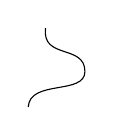
\begin{tikzpicture}[x=1cm,y=1cm,baseline=-.05cm]\draw[thin] (-.4,.6).. controls (-.45,.2) and (.1,.4)..(.1,.05).. controls (.1,-.25) and (-.6,-.05)..(-.62,-.4);\end{tikzpicture}}(k)$ be the category \deleted{of isocrystals} obtained from the category of \deleted{\unsure{cr|er}} nondegenerate $F$-cry\deleted{z}stals by localizing with respect to $p$ ; it is therefore a sub-$\otimes$-category of that of $F$-crystals up to isogeny. We shall call it the category of $F$-\uline{effective isocrystals}, and shall drop the qualifier ``iso'' if there is no risk of confusion.

% block: Tate crystal and inversion
\uline{The} $F$-\uline{inverse Tate\handwritten{\begin{tikzpicture}[x=1cm,y=1cm,baseline=-.05cm]\draw[thin] (-.1,-.4)--(.14,.45);\end{tikzpicture}} isocrystal}\inserted{$K(-1)$}\handwritten{\begin{tikzpicture}[x=1cm,y=1cm,baseline=-.1cm]\draw[thin] (0,.15).. controls (.05,-.1) and (-.2,-.1)..(-.7,-.1).. controls (-1,-.1) and (-1.3,-.2)..(-1.3,-.5);\end{tikzpicture}} is obtained from the $F$\handwritten{
\begin{tikzpicture}[x=1cm,y=1cm,baseline=-.05cm]\draw[thick] (.12,.3).. controls (-.1,.1) and (-.12,-.1)..(.12,-.26);\end{tikzpicture}}-crystal\inserted{$W(-1)$}\handwritten{\begin{tikzpicture}[x=1cm,y=1cm,baseline=-.1cm]\draw[thin] (0,.15).. controls (.05,-.1) and (-.2,-.1)..(-.7,-.1).. controls (-1,-.1) and (-1.3,-.2)..(-1.3,-.5);\end{tikzpicture}} defined by the \uline{unit} c\unsure{\deleted{y}r|\deleted{r}y}\unsure{\deleted{r}y|\deleted{y}r}stal, with $F_{K(-1)}=p.\operatorname{id}$ (this $F$-crystal is obviously nondegenerate !). One then sees that $K(-1)$ is weakly invertible, and one observes that when one formally adjoins to $\mathrm{FC}\overset{\handwritten{\mathord{\begin{tikzpicture}[x=1cm,y=1cm,baseline=0cm]\draw[thick] (0,0)--(.15,.015);\draw[thick] (.23,.025)--(.31,.005);\end{tikzpicture}}}}{\underset{r}{r}}\mathrm{iso}^{+}(k)$ \deleted{some} an in\handwritten{v}erse $K(1)$ of $K\handwritten{(-1),}$ then one obtains a Tannakian category over $\underline{Q}_p$, having an obvious fibre functor over $K$; this category is denoted $\operatorname{FCriso}(\unsure{\deleted{h}k|\deleted{k}h})$, and called the \uline{category of} $F$-\uline{\unsure{\deleted{c}i|\deleted{i}c}\unsure{\deleted{r}s|\deleted{s}r}ocrystals} \handwritten{(}or simply, if there \deleted{no} is no risk of confusion, of $F$-crystals) over $k$. $K(1)$ is the Tate $F$\handwritten{
\begin{tikzpicture}[x=1cm,y=1cm,baseline=-.05cm]\draw[thick] (.12,.3).. controls (-.1,.1) and (-.12,-.1)..(.12,-.26);\end{tikzpicture}}-crystal, and one denotes by $M\handwritten{\mapsto}M(n)$ the functor of tensoring with its $n$.th tensor power. If $n=-m$, $m\handwritten{\geqslant}0$, this func\deleted{t\unsure{o}}tor is induced by the functor on effective $F$-crystals (without iso\unsure{)} consisting in multiplying $F$ by $p^m$.

% block: crystals item 3
\handwritten{3.} When $k$ is perfect, denoting by $\handwritten{\sigma}$ the Frobenius automorphism of $W=W(k)$, giving an $F$-crystal amounts to giving a finitely generated module $M$ over $W$ equipped with a homomorphism
\[
F_M\handwritten{\unsure{\deleted{=}:|\deleted{:}=|\div}}\quad M^{\handwritten{\unsure{\deleted{\sigma}\sigma|\sigma}}}=M\otimes_W(W,\handwritten{\sigma})\handwritten{\longrightarrow}M\ ,
\]
and the $F$\handwritten{
\begin{tikzpicture}[x=1cm,y=1cm,baseline=-.05cm]\draw[thick] (.12,.3).. controls (-.1,.1) and (-.12,-.1)..(.12,-.26);\end{tikzpicture}}-crystal is nondegenerate if and only if the preceding homomorphism is an isogeny \unsure{\deleted{n}i|\deleted{i}n|i}.e. is of rank equal to $\operatorname{rang}M$, or again if and only if it induces an isomorphism after tensoring with $K$. The category \deleted{$\operatorname{Fiso}$} $\mathrm{Fc}\unsure{\deleted{\mathrm{ir}}\handwritten{ri}|\handwritten{ri}}\mathrm{s}(k)$ is then identified with the category of finite-dimensional vector spaces
% archive sheet number: 67
